\documentclass[12pt,a4paper]{article}
\usepackage[UTF8]{ctex}
\usepackage[margin=2.5cm]{geometry}
\usepackage{graphicx}
\usepackage{listings}
\usepackage{xcolor}
\usepackage{hyperref}
\usepackage{titlesec}
\usepackage{enumitem}
\usepackage{booktabs}
\usepackage{parskip}

% ────────────────────────────────────────────────────────────
%  颜色 & 代码风格
% ────────────────────────────────────────────────────────────
\definecolor{codebg}{RGB}{248,248,248}
\definecolor{codeframe}{RGB}{200,200,200}
\definecolor{diffadd}{RGB}{0,110,0}
\definecolor{diffdel}{RGB}{180,0,0}
\definecolor{diffhunk}{RGB}{0,60,160}
\definecolor{commentgray}{RGB}{100,100,100}

\lstdefinelanguage{diff}{
    morecomment=[f][\color{diffhunk}\bfseries]{@@},
    morecomment=[f][\color{diffdel}]{-},
    morecomment=[f][\color{diffadd}]{+}
}
\lstdefinestyle{diffstyle}{
    language=diff,
    backgroundcolor=\color{codebg},
    frame=single,
    rulecolor=\color{codeframe},
    basicstyle=\ttfamily\small,
    numbers=left,
    numberstyle=\tiny\color{gray},
    numbersep=8pt,
    tabsize=4,
    breaklines=true,
    showstringspaces=false,
    captionpos=b,
    xleftmargin=1em
}

\lstdefinestyle{cstyle}{
    language=C,
    backgroundcolor=\color{codebg},
    frame=single,
    rulecolor=\color{codeframe},
    basicstyle=\ttfamily\small,
    keywordstyle=\color{blue}\bfseries,
    commentstyle=\color{commentgray}\itshape,
    stringstyle=\color{orange!70!black},
    numbers=left,
    numberstyle=\tiny\color{gray},
    numbersep=8pt,
    tabsize=4,
    breaklines=true,
    showstringspaces=false,
    captionpos=b,
    xleftmargin=1em
}

\usepackage{titling}
\usepackage{tocloft}

% % --- 压缩 maketitle 的上下空白 ---
% \setlength{\droptitle}{-1.2cm}   % 标题整体上移
% \pretitle{\begin{center}\Large\bfseries}
% \posttitle{\par\end{center}}
% \preauthor{\begin{center}\normalsize}
% \postauthor{\par\end{center}}
% \predate{\begin{center}\small}
% \postdate{\par\end{center}}

% --- 压缩目录标题与条目间距 ---
\setlength{\cftbeforetoctitleskip}{0.2em}
\setlength{\cftaftertoctitleskip}{0.5em}
\setlength{\cftbeforesecskip}{0pt}   % 每个section目录项之间额外空白

% ────────────────────────────────────────────────────────────
%  标题信息
% ────────────────────────────────────────────────────────────
\title{%
  \textbf{操作系统实验报告}\\[0.4em]
  \large 第二次实验：uC/OS-II 时间片轮转调度器实现
}
\author{山东大学\ 网络空间安全学院\ 张宇杰}
\date{\today}

\begin{document}
\maketitle
{
\footnotesize 
\tableofcontents
}
\newpage

% ════════════════════════════════════════════════════════════
\section{实验概述}
% ════════════════════════════════════════════════════════════

本实验在 μC/OS-II 实时操作系统的基础上，分两个任务实现时间片轮转（Round-Robin）
调度机制：

\begin{itemize}
  \item \textbf{任务一}：为同一优先级的所有就绪任务实现单队列的时间片轮转调度，
        使相同优先级的任务能够公平地共享 CPU。
  \item \textbf{任务二（可选）}：在任务一的基础上扩展为\emph{分组}时间片轮转调度——
        每 8 个连续优先级为一组，共 8 组；组内实施轮转调度，组间仍按优先级调度。
\end{itemize}

实验涉及的主要文件如下表所示：

\begin{center}
\begin{tabular}{lll}
\toprule
文件 & 路径 & 主要修改内容 \\
\midrule
\texttt{main.c}      & 工程根目录              & 新增测试任务及其入口函数 \\
\texttt{os\_core.c}  & src/ucos\_ii/src/       & 就绪队列、调度器核心逻辑 \\
\texttt{os\_task.c}  & src/ucos\_ii/src/       & 任务删除时出队处理 \\
\texttt{ucos\_ii.h}  & src/ucos\_ii/src/       & 就绪队列全局变量声明 \\
\texttt{user\_asm.s} & 工程根目录              & 新增 \texttt{OSTaskDel} 系统调用 \\
\bottomrule
\end{tabular}
\end{center}

% ════════════════════════════════════════════════════════════
\section{任务一：单队列时间片轮转调度}
% ════════════════════════════════════════════════════════════

\subsection{设计思路}

原始 μC/OS-II 采用纯优先级抢占调度：每次调度总是选取优先级最高的就绪任务运行，
相同优先级的任务无法共享 CPU。为了实现时间片轮转，需要在不破坏优先级抢占语义
的前提下，对处于"当前最高优先级"的多个就绪任务维护一条 FIFO 就绪队列，并在每
次时钟中断时递减当前任务的剩余时间片，时间片耗尽时将该任务移到队尾，从队头取
下一个任务投入运行。

整体修改分为以下几个层次：

\begin{enumerate}
  \item 在 \texttt{os\_core.c} 中实现就绪队列的三个原语：\texttt{OSRdyQueueIn}、
        \texttt{OSRdyQueueOut}、\texttt{OS\_InitRdyQueue}。
  \item 在 \texttt{OSTimeTick} 中递减当前任务的剩余时间片，并在任务从阻塞态回到
        就绪态时将其入队。
  \item 修改 \texttt{OS\_SchedNew}，使时间片耗尽时执行轮转逻辑。
  \item 在 \texttt{OS\_TCBInit}（\texttt{OSTaskCreate} 的子程序）中对新建任务入队。
  \item 在 \texttt{OSTaskDel} 中对被删除的任务出队。
  \item 扩展 \texttt{main.c} 增加第三个测试任务，并通过 \texttt{user\_asm.s}
        暴露 \texttt{OSTaskDel} 的系统调用接口。
\end{enumerate}

% ────────────────────────────────────────────────────────────
\subsection{就绪队列实现（\texttt{os\_core.c}）}
% ────────────────────────────────────────────────────────────

就绪队列是一条带头尾指针的双向链表，利用 TCB 中新增的
\texttt{OSRdyTCBNext} 和 \texttt{OSRdyTCBPrev} 两个指针穿串。
三个全局变量（\texttt{OSRdyTCBQueueFront}、\texttt{OSRdyTCBQueueRear}、
\texttt{OSRdyTCBQueueNum}）分别记录队头、队尾和队列长度，均在
\texttt{ucos\_ii.h} 中以 \texttt{OS\_EXT} 宏声明，保证跨文件可见。

\subsubsection{\texttt{OS\_InitRdyQueue}——初始化就绪队列}

在系统启动时（\texttt{OSInit} 内）被调用，将队头、队尾置 NULL，队列长度归零。

\begin{lstlisting}[style=diffstyle,caption={os\_core.c — 就绪队列初始化}]
+void OS_InitRdyQueue(void)
+{
+    /* 队列为空：头尾指针都指向 NULL */
+    OSRdyTCBQueueFront = (OS_TCB *)0;
+    OSRdyTCBQueueRear  = (OS_TCB *)0;
+
+    /* 队列中没有任务 */
+    OSRdyTCBQueueNum   = 0;
+}
\end{lstlisting}

\subsubsection{\texttt{OSRdyQueueIn}——任务入队（队尾插入）}

当一个任务需要进入就绪队列时（新建、从阻塞态恢复、时间片耗尽后重新排队），
调用此函数。

\begin{itemize}
  \item 空闲任务（\texttt{OS\_TASK\_IDLE\_PRIO}）不参与轮转，直接返回。
  \item 重置该任务的剩余时间片为 \texttt{OS\_SCHED\_QUANTUM\_MAX}。
  \item 若队列为空，则新节点同时成为队头和队尾；否则链接到队尾并更新尾指针。
\end{itemize}

\begin{lstlisting}[style=diffstyle,caption={os\_core.c — 任务入队}]
+void OSRdyQueueIn(OS_TCB *ptcb)
+{
+    if (ptcb->OSTCBPrio == OS_TASK_IDLE_PRIO)
+        return;                   /* 空闲任务不进入轮转队列 */
+
+    ptcb->quantum      = OS_SCHED_QUANTUM_MAX;   /* 重置时间片 */
+    ptcb->OSRdyTCBNext = (OS_TCB *)0;
+    ptcb->OSRdyTCBPrev = (OS_TCB *)0;
+
+    if (OSRdyTCBQueueNum == 0) {
+        /* 队列为空，成为唯一节点 */
+        OSRdyTCBQueueFront = ptcb;
+        OSRdyTCBQueueRear  = ptcb;
+    } else {
+        /* 插入队尾 */
+        ptcb->OSRdyTCBPrev              = OSRdyTCBQueueRear;
+        OSRdyTCBQueueRear->OSRdyTCBNext = ptcb;
+        OSRdyTCBQueueRear               = ptcb;
+    }
+    OSRdyTCBQueueNum++;
+}
\end{lstlisting}

\subsubsection{\texttt{OSRdyQueueOut}——队头出队}

每次轮转时，从队头取出下一个将要运行的任务。若队列为空则返回 NULL；
若只有一个节点则队列归空；否则队头指针后移并清除新队头的前向指针。

\begin{lstlisting}[style=diffstyle,caption={os\_core.c — 队头出队}]
+OS_TCB *OSRdyQueueOut(void)
+{
+    OS_TCB *ptcb;
+
+    if (OSRdyTCBQueueFront == (OS_TCB *)0)
+        return (OS_TCB *)0;          /* 队列为空 */
+
+    ptcb = OSRdyTCBQueueFront;       /* 取出队头 */
+
+    if (OSRdyTCBQueueNum == 1) {
+        /* 只剩一个节点，队列变空 */
+        OSRdyTCBQueueFront = (OS_TCB *)0;
+        OSRdyTCBQueueRear  = (OS_TCB *)0;
+    } else {
+        /* 队头后移，清除新队头的前向指针 */
+        OSRdyTCBQueueFront               = ptcb->OSRdyTCBNext;
+        OSRdyTCBQueueFront->OSRdyTCBPrev = (OS_TCB *)0;
+    }
+    /* 清空出队节点的链表指针，避免悬空指针 */
+    ptcb->OSRdyTCBNext = (OS_TCB *)0;
+    ptcb->OSRdyTCBPrev = (OS_TCB *)0;
+    OSRdyTCBQueueNum--;
+    return ptcb;
+}
\end{lstlisting}

% ────────────────────────────────────────────────────────────
\subsection{时钟中断处理（\texttt{OSTimeTick}）}
% ────────────────────────────────────────────────────────────

\texttt{OSTimeTick} 在每次 SysTick 中断时被调用，负责维护时间相关的状态。
需要在此完成两件事：

\paragraph{递减当前任务的剩余时间片}

\begin{lstlisting}[style=diffstyle,caption={os\_core.c — 递减当前任务剩余时间片}]
 #if OS_SCHED_ROUND_ROBIN_EN > 0
+    if (OSTCBCur->quantum > 0) {
+        OSTCBCur->quantum--;   /* 每个时钟周期减 1；减到 0 时触发轮转 */
+    }
 #endif
\end{lstlisting}

\paragraph{阻塞态任务唤醒时入队}

原有代码已将解除阻塞的任务通过 \texttt{OSRdyGrp}/\texttt{OSRdyTbl}
标记为就绪，但轮转调度还需将其加入就绪队列。条件判断由框架提供：
若该任务此前不在就绪组/就绪位图中（即原来处于非就绪态），则现在入队。

\begin{lstlisting}[style=diffstyle,caption={os\_core.c — 阻塞转就绪时入队}]
 #if OS_SCHED_ROUND_ROBIN_EN > 0
     if ((OSRdyGrp & ptcb->OSTCBBitY) == 0 ||
         (OSRdyTbl[ptcb->OSTCBY] & ptcb->OSTCBBitX) == 0)
+        OSRdyQueueIn(ptcb);   /* 从阻塞态恢复的任务重新入就绪队列 */
 #endif
\end{lstlisting}

% ────────────────────────────────────────────────────────────
\subsection{调度器核心修改（\texttt{OS\_SchedNew}）}
% ────────────────────────────────────────────────────────────

\texttt{OS\_SchedNew} 负责决定下一个运行的任务（将结果写入全局变量
\texttt{OSPrioHighRdy}）。在轮转模式下，当当前任务时间片耗尽时，
需将其移到队尾并从队头选取下一个任务。

逻辑分两种情形：

\begin{enumerate}
  \item \textbf{系统刚启动（\texttt{OSTCBCur == 0}）}：尚无"当前任务"，
        直接按位图找最高优先级任务。
  \item \textbf{当前任务时间片耗尽（\texttt{quantum == 0}）}：
        先出队再入队（实现"移到队尾"），然后从队头取新任务的优先级；
        若队列为空（无同优先级可轮转的任务），回退到位图查找。
\end{enumerate}

\begin{lstlisting}[style=diffstyle,caption={os\_core.c — OS\_SchedNew 轮转逻辑}]
 #if OS_SCHED_ROUND_ROBIN_EN > 0
+    if (OSTCBCur == 0 | OSTCBCur->quantum == 0)
+    {
+        if (OSTCBCur != 0) {
+            OSRdyQueueOut();          /* 把当前任务从队头移走 */
+            OSRdyQueueIn(OSTCBCur);   /* 重新插入队尾，完成轮转 */
+        }
+        /* 选取下一个任务：优先从队列头部取，队列空则退回位图调度 */
+        if (OSRdyTCBQueueFront != (OS_TCB *)0) {
+            OSPrioHighRdy = OSRdyTCBQueueFront->OSTCBPrio;
+        } else {
+            INT8U y;
+            y = OSUnMapTbl[OSRdyGrp];
+            OSPrioHighRdy = (INT8U)((y << 3) + OSUnMapTbl[OSRdyTbl[y]]);
+        }
+    }
 #endif
\end{lstlisting}

% ────────────────────────────────────────────────────────────
\subsection{新建任务时入队（\texttt{OS\_TCBInit}）}
% ────────────────────────────────────────────────────────────

\texttt{OS\_TCBInit} 由 \texttt{OSTaskCreate} 调用，在 TCB 初始化完成后
将新任务加入就绪队列，使其能够参与后续的轮转调度。

\begin{lstlisting}[style=diffstyle,caption={os\_core.c — 新建任务入就绪队列}]
 #if OS_SCHED_ROUND_ROBIN_EN > 0
-    // your code:  put ptcb into queue of ready TCBs
+    OSRdyQueueIn(ptcb);   /* 新建任务加入轮转就绪队列 */
 #endif
\end{lstlisting}

% ────────────────────────────────────────────────────────────
\subsection{任务删除时出队（\texttt{os\_task.c}）}
% ────────────────────────────────────────────────────────────

当一个任务主动调用 \texttt{OSTaskDel} 删除自身时，必须将其从就绪队列中
移除，否则轮转队列中将保留悬空的 TCB 指针，导致非法内存访问。

\begin{lstlisting}[style=diffstyle,caption={os\_task.c — 任务删除时出队}]
 #if OS_SCHED_ROUND_ROBIN_EN > 0
+    OSRdyQueueOut();   /* 从轮转就绪队列中移除当前任务 */
+    OSTCBCur = 0;      /* 清空当前任务指针，触发重新调度 */
 #endif
\end{lstlisting}

将 \texttt{OSTCBCur} 置零后，下一次 \texttt{OS\_SchedNew} 进入
\texttt{OSTCBCur == 0} 分支，系统将正确地从队列或位图中选取新任务。

% ────────────────────────────────────────────────────────────
\subsection{扩展系统调用——\texttt{OSTaskDel}（\texttt{user\_asm.s}）}
% ────────────────────────────────────────────────────────────

为了让运行在非特权模式下的用户任务能够调用 \texttt{OSTaskDel}，
需要在汇编层面扩展 SVC（系统调用）分派表，分配新的调用号 \texttt{0x06}。

\subsubsection{导入/导出声明}

\begin{lstlisting}[style=diffstyle,caption={user\_asm.s — 新增 OSTaskDel 导入导出}]
 IMPORT OSTaskCreate
+IMPORT OSTaskDel
 EXPORT syscall_OSTaskCreate
+EXPORT syscall_OSTaskDel
\end{lstlisting}

\subsubsection{SVC 分派}

在 \texttt{SVC\_Handler} 中增加对调用号 \texttt{0x06} 的判断：

\begin{lstlisting}[style=diffstyle,caption={user\_asm.s — SVC 分派新增 OSTaskDel}]
     CMP   R0, #0x05
     BEQ   OSTaskCreate_call
+    CMP   R0, #0x06
+    BEQ   OSTaskDel_call
     BX    LR
\end{lstlisting}

\subsubsection{OSTaskDel 调用桩}

\begin{lstlisting}[style=diffstyle,caption={user\_asm.s — OSTaskDel 调用桩实现}]
+OSTaskDel_call
+    LDR   R0, [R2]       ; 从用户栈加载参数（优先级号）
+    MOV   R1, #0xFFFF
+    AND   R0, R1         ; 截取低 16 位，确保参数合法
+    PUSH  {LR}
+    BL    OSTaskDel      ; 调用内核函数
+    POP   {LR}
+    BX    LR
\end{lstlisting}

\subsubsection{用户侧包装函数}

\begin{lstlisting}[style=diffstyle,caption={user\_asm.s — syscall\_OSTaskDel 用户包装}]
+syscall_OSTaskDel
+    SWI 0x06    ; 触发 SVC，调用号 0x06
+    BX  LR
\end{lstlisting}

% ────────────────────────────────────────────────────────────
\subsection{测试用例（\texttt{main.c}）}
% ────────────────────────────────────────────────────────────

在原有两个任务的基础上新增 Task 3，三个任务具有相同优先级，
用于验证时间片轮转是否正常工作。每个任务循环打印 9 次后调用
\texttt{syscall\_OSTaskDel} 退出。

\begin{lstlisting}[style=diffstyle,caption={main.c — 新增第三个测试任务}]
 static OS_STK task2_stk[TASK1_STK_SIZE];
+static OS_STK task3_stk[TASK1_STK_SIZE];
 void task1(void *p_arg);
 void task2(void *p_arg);
+void task3(void *p_arg);
+INT8U  syscall_OSTaskDel (INT8U prio);
\end{lstlisting}

\begin{lstlisting}[style=diffstyle,caption={main.c — 在 main() 中创建 Task 3 并修改各任务逻辑}]
+    OSTaskCreate(task3, (void *)0,
+        &task3_stk[TASK3_STK_SIZE - 1], TASK3_PRIO);

+static void task1(void *p_arg)
+{
+    for (int i = 1; i < 10; i++) {
+        syscall_print_str("Hello from Task 1!\n");
+    }
+    syscall_OSTaskDel(OS_PRIO_SELF);  /* 完成后删除自身 */
+}

 /* task2 和 task3 结构类似，分别打印 Task 2 / Task 3 标识后自删 */
\end{lstlisting}

在上述测试中，三个任务共享同一优先级，预期输出应交替出现
\texttt{Task 1 / Task 2 / Task 3}，每轮切换恰好在一个时间片
（\texttt{OS\_SCHED\_QUANTUM\_MAX} 个 tick）之后发生，
从而验证轮转调度的正确性。

经调试，调度器正确工作，三个task正确轮换，在task1退出后，剩余两个task也正确轮换：

\begin{figure}[htbp]
    \centering
    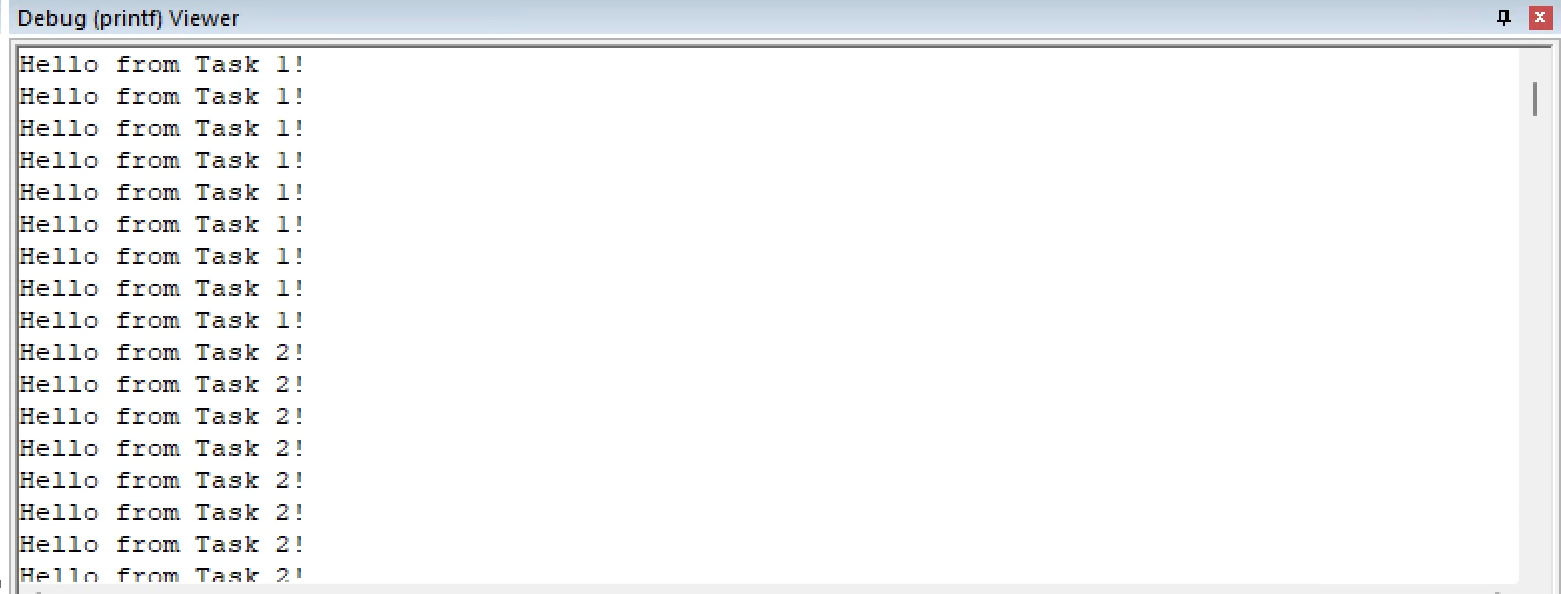
\includegraphics[width=0.8\linewidth]{figure/task1.png}
\end{figure}

% ════════════════════════════════════════════════════════════
\section{任务二：分组时间片轮转调度（可选）}
% ════════════════════════════════════════════════════════════

\subsection{设计思路}

任务二在任务一的基础上将轮转调度的范围限制在\emph{同一优先级组}内：
μC/OS-II 将 0--63 号优先级按每 8 个一组分为 8 组（组号 = 优先级 >> 3）。
组间依然按优先级高低抢占，组内各任务轮转。

关键改动是将任务一中的单条就绪队列（\texttt{OSRdyTCBQueueFront} 等）
扩展为 8 条队列（下标即组号），并修改 \texttt{OSRdyQueueIn} /
\texttt{OSRdyQueueOut} / \texttt{OS\_SchedNew} 的相应逻辑。

% ────────────────────────────────────────────────────────────
\subsection{全局变量修改（\texttt{ucos\_ii.h}）}
% ────────────────────────────────────────────────────────────

将单条队列的头尾指针和计数器替换为各含 8 个元素的数组：

\begin{lstlisting}[style=diffstyle,caption={ucos\_ii.h — 就绪队列全局变量扩展为 8 组}]
 #if OS_SCHED_ROUND_ROBIN_EN > 0
-OS_EXT  OS_TCB           *OSRdyTCBQueueFront;
-OS_EXT  OS_TCB           *OSRdyTCBQueueRear;
-OS_EXT  INT8U             OSRdyTCBQueueNum;
+OS_EXT  OS_TCB           *OSRdyTCBQueueFrontTbl[8];  /* 每组队头 */
+OS_EXT  OS_TCB           *OSRdyTCBQueueRearTbl[8];   /* 每组队尾 */
+OS_EXT  INT8U             OSRdyTCBQueueNumTbl[8];    /* 每组队列长度 */
 #endif
\end{lstlisting}

% ────────────────────────────────────────────────────────────
\subsection{就绪队列原语修改（\texttt{os\_core.c}）}
% ────────────────────────────────────────────────────────────

\subsubsection{\texttt{OS\_InitRdyQueue}——批量清零}

使用 \texttt{OS\_MemClr} 对三个数组整体清零，比逐项赋值更简洁：

\begin{lstlisting}[style=diffstyle,caption={os\_core.c — 分组队列初始化}]
 void OS_InitRdyQueue(void)
 {
+    OS_MemClr((INT8U *)&OSRdyTCBQueueFrontTbl[0], sizeof(OSRdyTCBQueueFrontTbl));
+    OS_MemClr((INT8U *)&OSRdyTCBQueueRearTbl[0],  sizeof(OSRdyTCBQueueRearTbl));
+    OS_MemClr((INT8U *)&OSRdyTCBQueueNumTbl[0],   sizeof(OSRdyTCBQueueNumTbl));
 }
\end{lstlisting}

\subsubsection{\texttt{OSRdyQueueIn}——按组入队}

通过 TCB 中已有的字段 \texttt{OSTCBY}（= 优先级 >> 3）确定所属组号，
后续逻辑与任务一完全相同，只是操作对象从单条队列变为对应组的队列：

\begin{lstlisting}[style=diffstyle,caption={os\_core.c — 按组入队}]
 void OSRdyQueueIn(OS_TCB *ptcb)
 {
+    INT8U grp;
     if (ptcb->OSTCBPrio == OS_TASK_IDLE_PRIO)
         return;
+    grp = ptcb->OSTCBY;   /* 优先级组号 = 优先级 >> 3 */

+    ptcb->quantum      = OS_SCHED_QUANTUM_MAX;
+    ptcb->OSRdyTCBNext = (OS_TCB *)0;
+    ptcb->OSRdyTCBPrev = (OS_TCB *)0;

+    if (OSRdyTCBQueueNumTbl[grp] == 0) {
+        OSRdyTCBQueueFrontTbl[grp] = ptcb;
+        OSRdyTCBQueueRearTbl[grp]  = ptcb;
+    } else {
+        ptcb->OSRdyTCBPrev                     = OSRdyTCBQueueRearTbl[grp];
+        OSRdyTCBQueueRearTbl[grp]->OSRdyTCBNext = ptcb;
+        OSRdyTCBQueueRearTbl[grp]              = ptcb;
+    }
+    OSRdyTCBQueueNumTbl[grp]++;
 }
\end{lstlisting}

\subsubsection{\texttt{OSRdyQueueOut}——按组出队}

签名改为接受组号参数 \texttt{grp}，逻辑与任务一类似：

\begin{lstlisting}[style=diffstyle,caption={os\_core.c — 按组出队（签名变更）}]
-OS_TCB *OSRdyQueueOut(void)
+OS_TCB *OSRdyQueueOut(INT8U grp)
 {
     OS_TCB *ptcb;
+    if (OSRdyTCBQueueFrontTbl[grp] == (OS_TCB *)0)
         return (OS_TCB *)0;
+    ptcb = OSRdyTCBQueueFrontTbl[grp];
+    if (OSRdyTCBQueueNumTbl[grp] == 1) {
+        OSRdyTCBQueueFrontTbl[grp] = (OS_TCB *)0;
+        OSRdyTCBQueueRearTbl[grp]  = (OS_TCB *)0;
+    } else {
+        OSRdyTCBQueueFrontTbl[grp]               = ptcb->OSRdyTCBNext;
+        OSRdyTCBQueueFrontTbl[grp]->OSRdyTCBPrev = (OS_TCB *)0;
+    }
     ptcb->OSRdyTCBNext = (OS_TCB *)0;
     ptcb->OSRdyTCBPrev = (OS_TCB *)0;
+    OSRdyTCBQueueNumTbl[grp]--;
     return ptcb;
 }
\end{lstlisting}

% ────────────────────────────────────────────────────────────
\subsection{调度器修改（\texttt{OS\_SchedNew}）}
% ────────────────────────────────────────────────────────────

组间优先级调度通过 \texttt{OSRdyGrp}/\texttt{OSRdyTbl} 位图确定最高优先
级组号 \texttt{y}，再在该组内进行轮转：

\begin{lstlisting}[style=diffstyle,caption={os\_core.c — 分组轮转调度逻辑}]
 #if OS_SCHED_ROUND_ROBIN_EN > 0
+    if (OSTCBCur == 0)
+    {
+        INT8U y;
+        y = OSUnMapTbl[OSRdyGrp];         /* 最高优先级组号 */
+        OSPrioHighRdy = (INT8U)((y << 3) + OSUnMapTbl[OSRdyTbl[y]]);
+    }
+    else if (OSTCBCur->quantum == 0)
+    {
+        INT8U y;
+        y = OSUnMapTbl[OSRdyGrp];         /* 当前最高优先级组号 */
+
+        if (OSTCBCur->OSTCBPrio != OS_TASK_IDLE_PRIO)
+        {
+            OSRdyQueueOut(OSTCBCur->OSTCBY);  /* 从本组队列移走当前任务 */
+            OSRdyQueueIn(OSTCBCur);           /* 重新入本组队尾 */
+            /* 从最高优先级组的队头取下一个任务 */
+            OSPrioHighRdy = OSRdyTCBQueueFrontTbl[y]->OSTCBPrio;
+        }
+        else
+        {
+            /* 空闲任务：回退到位图调度 */
+            OSPrioHighRdy = (INT8U)((y << 3) + OSUnMapTbl[OSRdyTbl[y]]);
+        }
+    }
 #endif
\end{lstlisting}

关键区别在于出队时传入的是\emph{当前任务所在的组}（\texttt{OSTCBCur->OSTCBY}），
而选取下一任务时使用的是\emph{当前最高优先级组}（\texttt{y}）——
这两者在组间出现更高优先级任务时会不同，从而保证组间抢占正确工作。

% ────────────────────────────────────────────────────────────
\subsection{任务删除适配（\texttt{os\_task.c}）}
% ────────────────────────────────────────────────────────────

由于 \texttt{OSRdyQueueOut} 的签名已改为接受组号，删除任务时
需传入被删除任务的组号：

\begin{lstlisting}[style=diffstyle,caption={os\_task.c — 任务删除出队（传入组号）}]
 #if OS_SCHED_ROUND_ROBIN_EN > 0
-    OSRdyQueueOut();
+    OSRdyQueueOut(ptcb->OSTCBY);  /* 按组号出队 */
     OSTCBCur = 0;
 #endif
\end{lstlisting}

% ────────────────────────────────────────────────────────────
\subsection{测试用例扩展（\texttt{main.c}）}
% ────────────────────────────────────────────────────────────

任务二新增 Task 4 和 Task 5，分配到不同的优先级组，
以验证组间优先级抢占与组内轮转能够同时正确工作。

\begin{lstlisting}[style=diffstyle,caption={main.c — 任务二测试任务（5 个任务，跨组）}]
+static OS_STK task4_stk[TASK1_STK_SIZE];
+static OS_STK task5_stk[TASK1_STK_SIZE];
 void task4(void *p_arg);
 void task5(void *p_arg);

     OSTaskCreate(task3, (void *)0, &task3_stk[...], 9);   /* 组 1 */
+    OSTaskCreate(task4, (void *)0, &task4_stk[...], 11);  /* 组 1，与 task3 轮转 */
+    OSTaskCreate(task5, (void *)0, &task5_stk[...], 22);  /* 组 2，优先级低于组 1 */
\end{lstlisting}

其中 Task 1（prio = TASK1\_PRIO）和 Task 2（prio = TASK2\_PRIO）
若在同一组内，则两者轮转；Task 3 与 Task 4 均在第 1 组（优先级 9 和 11），
两者也轮转；Task 5 在第 2 组（优先级 22），只有高优先级组任务全部退出后
才会被调度，用于验证组间抢占。

Task 5 设计为无限循环以观察低优先级任务在更高优先级组任务退出后才获得 CPU：

\begin{lstlisting}[style=diffstyle,caption={main.c — task5 无限循环（低优先级验证）}]
+static void task5(void *p_arg)
+{
+    int i;
+    for (;;)
+    {
+        for (i = 1; i < 10; i++)
+            ;
+        syscall_print_str("Hello from Task 5!\n");
+    }
+}
\end{lstlisting}

经调试，调度器正确工作，在task1,task2都退出后，正确的找到了优先级最高的组，并正确的轮换了组里的task：

\begin{figure}[htbp]
    \centering
    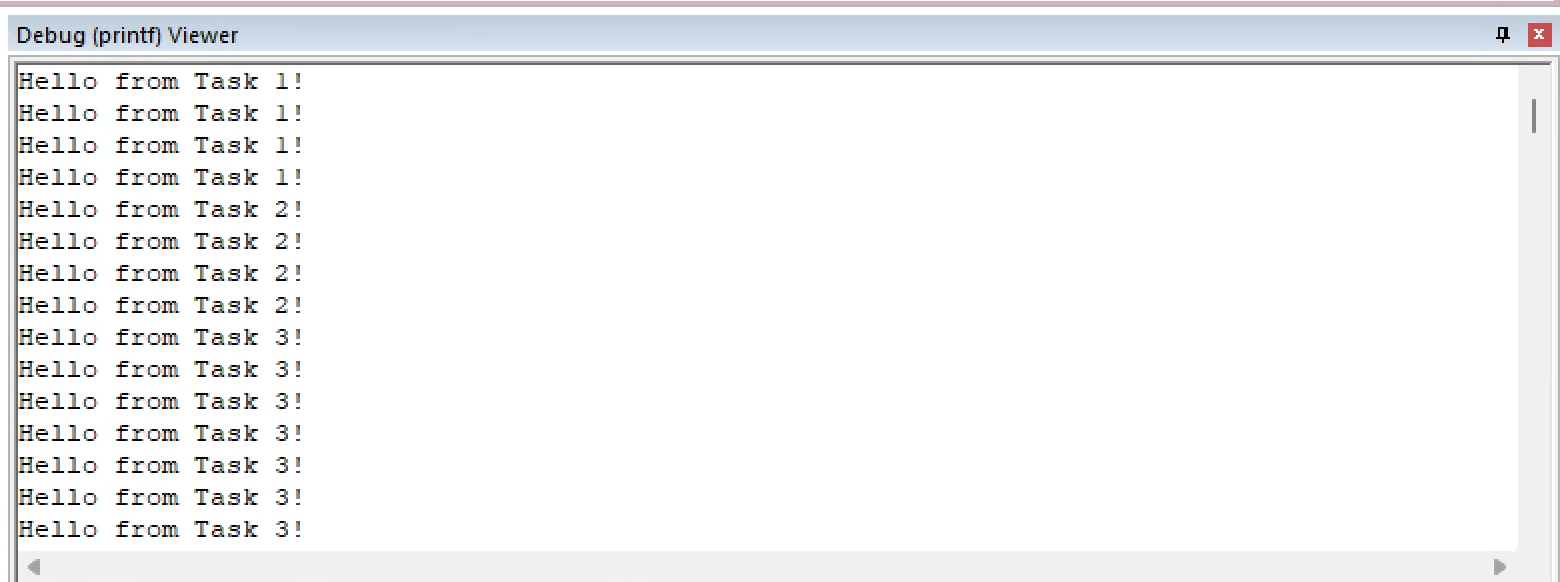
\includegraphics[width=0.8\linewidth]{figure/task2.png}
\end{figure}

% ════════════════════════════════════════════════════════════
\section{总结}
% ════════════════════════════════════════════════════════════

本次实验在 μC/OS-II 的基础上实现了两个层次的时间片轮转调度扩展：

\begin{itemize}
  \item \textbf{任务一}将全体就绪任务组织为一条 FIFO 双向链表，
        每个时钟中断递减当前任务剩余时间片，时间片耗尽后执行"先出后入"
        的轮转操作，并修改 \texttt{OS\_SchedNew} 从队头而非位图选取下一任务。
        同时扩展了 \texttt{OSTaskDel} 的系统调用路径，使非特权模式下的任务
        能够主动退出并安全地将自身从队列中移除。

  \item \textbf{任务二}将单条队列扩展为按优先级组索引的 8 条队列，
        在不影响组间优先级抢占语义的前提下，让同一组内的任务轮流共享 CPU，
        是对任务一数据结构和调度逻辑的自然推广。
\end{itemize}

两次改动均以条件编译宏 \texttt{OS\_SCHED\_ROUND\_ROBIN\_EN}
控制，对原有优先级调度路径无侵入。

\end{document}